\section{Experiments}

%To assess the efficacy of our proposed technique, we have conduct experiments to address the following research question: \textit{Does combining latent and meta path-based topological features improve relationship prediction accuracy in DHINs?}


\subsection{Experiment Setup}

\subsubsection{Dataset.} We conduct our experiments on two real-world network datasets that have different characteristics and evolution behaviour. 

\textit{Publications dataset:} The AMiner citation dataset \cite{Tang:08KDD} version 8 (2016-07-14) is extracted from DBLP, ACM, and other sources. It contains 3,272,991 papers and 8,466,859 citation relationships for 1,752,443 authors, who published in 10,436 venues, from 1936 to 2016. Each paper is associated with an abstract, authors, year, venue, and title. We confined our experiments on papers published since 1996, which includes 2,935,679 papers. Similar to \cite{sun2011ASONAM}, we considered only authors with at least 5 papers.
    
\textit{Movies dataset:} The RecSys HetRec movie dataset \cite{Cantador:RecSys2011} is an extension of MovieLens10M dataset, published by the GroupLens research group that links the movies of MovieLens dataset with their corresponding web pages on IMDB and Rotten Tomatoes. It contains information of 2,113 users, 10,197 movies, 20 movie genres (avg. 2.04 genres per movie), 4,060 directors, 95,321 actors (avg. 22.78 actors per movie), 72 countries, and 855,598 ratings (avg. 404.92 ratings per user, and avg. 84.64 ratings per movie).%, and 13,222 tags (avg. 22.69 tags per user, avg. 8.12 tags per movie).


\subsubsection{Experiment Settings.} We describe meta paths and target relationships, baseline methods, and different parameter settings.

\textit{Meta Paths and Target Relationships}. Figure \ref{Fig:expSchema} depicts network schemas for the two datasets. Note that we consider a simplified version and ignore nodes such as topic for papers or tag for movies. Table \ref{tbl:mp} presents a number of meta paths that we consider in our experiments, where target meta path relations are \textit{co-authorship} and \textit{watching}. 
%We also limit our meta path-based measures to only path count for calculations efficiency, as the results in \cite{sun2011ASONAM} suggest that except for the case of hybrid features, using the path count measure is not considerably different than the normalized path count or the random walk. %Note that the goal of our research is not to select the best features but to show the strength of combining meta paths with temporal latent features.


\begin{figure}[t]
\centering
\subfigure[Publications Network]{
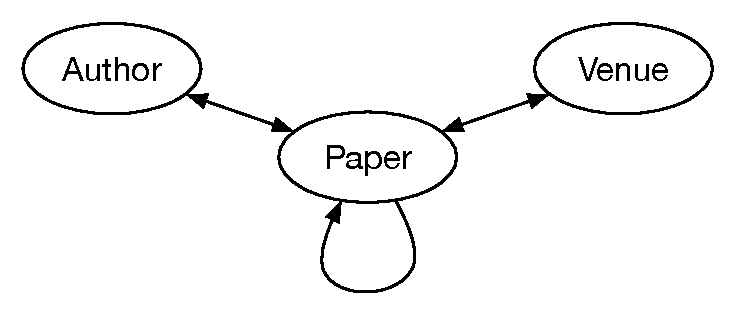
\includegraphics[trim = 0mm 0mm 0mm 0mm,width=0.44\hsize]{figs/publicationsSchema.pdf}
 \label{Fig:DBLP}
}
\subfigure[Movies Network]{
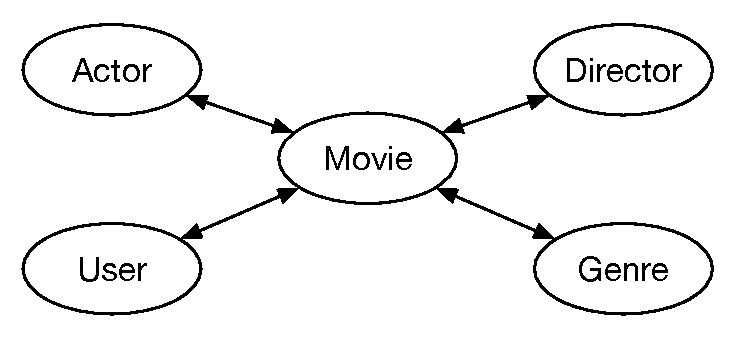
\includegraphics[trim = 0mm 0mm 0mm 0mm,width=0.44\hsize]{figs/moviesSchema.pdf}
 \label{Fig:IMDB}
}
\caption{The simplified network schema used for our experiments.} \label{Fig:expSchema}
\end{figure}


\begin{table}[t]
\centering
\caption{Meta paths for publications dataset with $V$=\{Author, Paper, Venue\} and movies dataset with $V$=\{User, Movie, Actor, Director, Genre\}.}
\label{table_publications}\label{tbl:mp}
\begin{tabular}{|l|c|l|} \hline
\textbf{Network} & \textbf{Meta path} & \textbf{Meaning} \\ \hline\hline

\multirow{4}{*}{Publications} & \textit{A--P--A} & [\textit{The target relation}] Authors are coauthors \\ \cline{2-3}
& \textit{A--P--V--P--A} & Authors publish in the same venue \\ \cline{2-3}
& \textit{A--P--A--P--A} & Authors have the same co-author \\ \cline{2-3}
& \textit{A--P--P--P--A} & Authors cite the same papers \\ \hline\hline

\multirow{5}{*}{Movies} & \textit{U--M} & [\textit{The target relation}] A user watches a movie \\ \cline{2-3}
& \textit{U--M--A--M} & A user watches a movie with the same actor \\ \cline{2-3}
& \textit{U--M--D--M} & A user watches a movie with the same director \\ \cline{2-3}
& \textit{U--M--G--M} & A user watches a movie of the same genre \\ \cline{2-3}
& \textit{U--M--U--M} & A user watches a movie that another user  \\ \hline

\end{tabular}
\end{table}

%For the publications network we consider meta paths \textit{A-P-V-P-A}, \textit{A-P-A-P-A}, and \textit{A-P-P-P-A}, as the study in \cite{sun2011ASONAM} shows that shared co-authors, shared venues, and co-cited papers for two authors significantly contribute to their future collaborations. There are two major differences between target relation types in our datasets. First, unlike a new co-authorship relation that happens at a particular time, users can watch/rate a movie once it is released. In other words each paper is published once and a new co-authorship is made at that time whereas users create new watching relations to an existing movie. Second, the target relation for the publications dataset, i.e., \textit{A-P-A}, has the same node type at both ends, while the target meta path for the movie dataset, i.e., \textit{U-M}, considers two different node types. Note that $G^\mathcal{P}_i$s in Equation 1 are square adjacency matrices. For the case of having target relations with two types of nodes at ends, we consider 0 value for the relationships of the same type in case no such relation actually exists in the network.

%to show the effectiveness of our proposed methods in predicting such relationships. 


%conducted Wald test in a case study and found that the $p$-value for the feature associated with each meta path and their significance level. From the results, we can see that the 

% Movies
%Out of 12310, 10109 movies were rated movies



\textit{Baseline Methods.} Sun et al. \cite{sun2011ASONAM} proposed a supervised learning framework for link prediction in HINs, called {PathPredict}, that learns coefficients associated with meta path-based features by maximizing the likelihood of new relationship formation. Their model is learned based on one past interval and does not consider temporal changes in different intervals. We perform comparative analysis of our work, denoted as {MetaDynaMix}, with four techniques: (1) The original {PathPredict} that considers only 3 intervals, (2) PathPredict applied on different time intervals, denoted as {PathPredict+}, (3) homogenized link prediction (Section \ref{def:HLP}), denoted as {HLP}, and (4) logistic regression on HLP latent features, denoted as {LRHLP}. %The state-of-the-art methods which we compare against are \textit{PathPredict} \cite{sun2011ASONAM}, and matrix factorization for temporal prediction \cite{Zhu2016} (denoted as \textit{BCGD}). 
The authors in \cite{sun2011ASONAM} showed that {PathPredict} outperforms traditional link prediction approaches that use topological features defined in homogeneous networks such as common neighbors or Katz$\beta$, and thus we do not include these techniques in our experiments.


%\begin{itemize}
%    \item  Heterogeneous non-temporal (PathCount, PathSim, NormalPathCount, RandomWalk, SymmetricRandomWalk)
%    \item  Homogeneous non-temporal (Katz, Jaccard)
%    \item  Homogeneous temporal (BCGD)
%\end{itemize}


\textit{Parameters.} We set the number of snapshots $t$=3, 5, and 7 to evaluate the effect of dynamic analysis of different time intervals. Note that $t$=3 refers to the default case for many link prediction algorithms that learn based on one interval and test based on another. More specifically in the training phase features are extracted based on T1 and labels are determined based on T2, and for the testing phase features are calculated based on T2 and labels are derived from T3. In our experiments we did not observe a considerable change in prediction performance by setting the number of latent features $k$ to 5, 10, and 20, and thus all presented results are based on setting $k$ to 20. %We also evaluate the effect of latent space dimensionality by setting the number of latent features $k$ to 5, 10, and 20.

\subsubsection{Implementation.} We use the implementation of matrix factorization for inferring temporal latent spaces of a sequence of graph snapshots presented in \cite{Zhu2016}. We use all the default settings such as the number of latent features $k$ to be 20, and the optimization algorithm to be the local block-coordinate gradient descent. For the classification part, we use the efficient LIBLINEAR \cite{fan2008liblinear} package and set the type of solver to L2-regularized logistic regression (primal). %that solves $min_w w^Tw/2 + C \sum log(1 + exp(-y_i w^Tx_i))$, where $w$ is the generated weight vector as the model for a given set of instance-label pairs $(x_i, y_i)$, $i$ = 1, . . . , l, $x_i \in R^n$, $y_i \in \{-1, +1\}$,  $w^Tw/2$ is the regularization term, and $C > 0$ is a penalty parameter. In the testing phase, we predict a data point $x$ as positive if $w^Tx > 0$, and negative otherwise.


\subsubsection{Evaluation Metrics.} 

To asses link prediction performance, we use Area Under Curves (AUC) for Receiver Operating Characteristic (ROC) \cite{davis2006relationship} %and Precision-Recall (PR) \cite{davis2006relationship}, 
and accuracy (ACC). %We also present the prediction accuracy for 5-fold cross validation. 
We also perform the McNemar's test \cite{mcnemar1947note} to assess the statistical significance of the difference between classification techniques.

\subsection{Results and Findings}

\textit{Link Prediction Accuracy}. In this part we compare the prediction accuracy of different methods. The  results shown in Figure \ref{fig:auc} are based on setting the number of time intervals $t$ to 7 for dynamic methods and 3 intervals for PathPredict. Table \ref{tbl:auc} shows more details considering different intervals. These results indicate the statistically significant improvement provided by the proposed MetaDynaMix prediction method compared to the baselines. The authors in \cite{menon2011link,Zhu2016} showed that latent features are more predictive compared to unsupervised scoring techniques such as Katz, or Adamic. In our experiments we observed that combining latent with meta path-based features (MetaDynaMix) can increase prediction accuracy. However, if latent features learn similar structure as topological features do, then mixing them may not be beneficial. In such cases feature engineering techniques could be applied. 

We also observe that PathPredict+ performs better than LRHLP in predicting links for the publications network but LRHLP predicts more accurate on the movies network. This implies that unlike the publications network, our meta path-based features for the movies network are not as predictive as latent features. However, in both cases combining the two set of features improves the performance.

%\ebrahim{If you are raising this point, then you have to also say why pp+ does not work well on movie dataset?Also, I could not see how the justification to combine features was reached. You may want to discuss more.}

%Adding more features to our Logistic Regression model will increase the training accuracy because model has to consider more data to fit the logistic regression. But testing accuracy increases if feature is found to be significant


\begin{figure}[t]
\centering
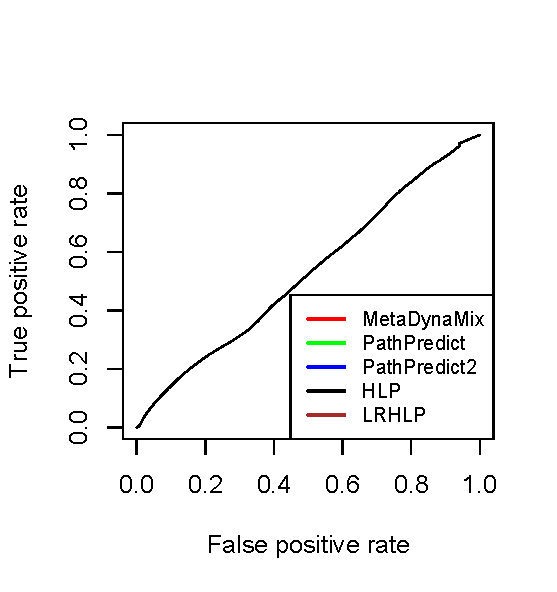
\includegraphics[trim = 0mm 10mm 0mm 0mm,width=0.86\textwidth]{figs/ROC.pdf}
\caption{The ROC curves for different methods and datasets.} \label{fig:auc}
\end{figure}


%\begin{figure}[t]
%\centering
%\subfigure[Publications Network]{
%\includegraphics[trim = 0mm 3mm 0mm 0mm,width=0.8\hsize]{figs/DBLP_AUC.pdf}
% \label{Fig:DBLP2}
%}
%\subfigure[Movies Network]{
%\includegraphics[trim = 0mm 3mm 0mm 10mm,width=0.8\hsize]{figs/IMDB_AUC.pdf}
% \label{Fig:IMDB}
%}
%\caption{The ROC curves for different methods and datasets.} \label{fig:auc}
%\end{figure}


\begin{table}[t]
\centering
\caption{Relationship prediction accuracy comparison. Bold values are determined to be statistically significant compared to the baselines based on McNemar's test.}
\label{table_publications}\label{tbl:auc}
\begin{tabular}{ll|p{1cm}|p{1cm}|p{1cm}||p{1cm}|p{1cm}|p{1cm}|}
\cline{3-8}
                        &   & \multicolumn{3}{l||}{Publications Network} & \multicolumn{3}{l|}{Movies Network} \\ \hline
\multicolumn{1}{|l|}{\textbf{Method}} & \textbf{Metric} & $t$=3 & $t$=5  & $t$=7  & $t$=3  & $t$=5  & $t$=7     \\ \hline\hline

\multicolumn{1}{|l|}{\multirow{2}{*}{PathPredict}}  & ROC  & 0.78 & -- & -- & 0.56 & -- & -- \\ \cline{2-8}
%\multicolumn{1}{|l|}{}  & PR  & 0.45 & -- & -- & 0.45 & -- & -- \\ \cline{2-8}
\multicolumn{1}{|l|}{}  & ACC  & 0.55 & -- & -- & 0.54  & -- & -- \\ \hline\hline

\multicolumn{1}{|l|}{\multirow{2}{*}{PathPredict+}}  & ROC  &  0.78  &   0.80    &     0.83    &   0.56   &    0.57     &    0.57     \\ \cline{2-8}
%\multicolumn{1}{|l|}{}  & PR  &   0.45  &    0.45    &   0.45   &   0.45  &     0.45    &     0.46    \\ \cline{2-8}
\multicolumn{1}{|l|}{}  & ACC  & 0.55  & 0.58  &  0.60 & 0.54  &  0.54  & 0.55   \\ \hline\hline

\multicolumn{1}{|l|}{\multirow{2}{*}{HLP}}  & ROC  &   0.42  &   0.43   &   0.46     &     0.51    &    0.53     &    0.54     \\ \cline{2-8}
%\multicolumn{1}{|l|}{}  & PR  &    0.43  &   0.44   &   0.45    &   0.44   &  0.45   &  0.45  \\ \cline{2-8}
\multicolumn{1}{|l|}{}  & ACC  & 0.50  &  0.50  &  0.50 &  0.51  &  0.52  &  0.53  \\ \hline\hline

\multicolumn{1}{|l|}{\multirow{2}{*}{LRHLP}}  & ROC  &   0.49   &   0.50   &   0.52    &    0.52     &   0.56   &   0.59      \\ \cline{2-8}
%\multicolumn{1}{|l|}{}  & PR  &  0.45    &   0.45   &   0.45   &  0.45   &   0.45   &   0.45      \\ \cline{2-8}
\multicolumn{1}{|l|}{}  & ACC  & 0.47 & 0.50  & 0.51   & 0.52  & 0.56  &  0.58  \\ \hline\hline

\multicolumn{1}{|l|}{\multirow{2}{*}{MetaDynaMix}}  & ROC  & 0.85 &  0.87 & \textbf{0.87}   &  0.57  & 0.59 &  \textbf{0.63}  \\ \cline{2-8}
%\multicolumn{1}{|l|}{}  & PR  & 0.46 &  0.46  &  \textbf{0.46}  &  0.46 &  0.46  & \textbf{0.47}   \\ \cline{2-8}
\multicolumn{1}{|l|}{}  & ACC  & 0.78 & 0.80 & \textbf{0.82}   & 0.56  &  0.60  &   \textbf{0.62} \\ \hline

\end{tabular}
\end{table}


%percentage
%91: our acc for min5 at t=7
%60: pathpred2 acc for min5 at t=7
%50: LRHLP



\textit{Significance of Performance Improvement}. McNemar's test, also called within-subjects $\chi^2$ test, is used to compare statistically significant difference between the accuracy of two predictive models based on the contingency table of their predictions. The null hypothesis indicates that the performances of the two models are equal. We compare MetaDynaMix with the other four baselines and the test results show a $p$-value $<$ 0.0001 for all cases and hence we reject the null hypothesis.

%DBLP
%    179,607 authors had no co-author in 1996-2016. 
%    78,635 authors had no co-author (about 4\%). 
%    ------------
%    100,972 (those who published in 1930-1996)?
%    
%    1,752,443 (total) - 100,972 = 1,651,471 (those who published in 1996-2016)?
%    
%    1,544,408 authors had no co-author in 1930-1996
%    78,635 authors had no co-author (about 4\%). 
%    ------------
%    1,465,773 (those who published in 1996-2016)?
%
%    1,752,443 (total) -1,465,773 = 300,000 (those who published in between)?
    
%    1,752,443 author_papervenuelist_map
%    2,811,533 paper_authorslist_map
%    10,163 venue_paperauthorslist_map
    
%78,635 authors had no co-author (about 4\%)


\textit{The Effect of Time Intervals}. We set the number of time intervals $t$ to 3, 5, and 7 and assess its impact on prediction performance. As presented in Table \ref{tbl:auc}, accuracy increases with the number of snapshots. The intuition is that shorter time interval results in less changes in the graph and thus leads to more reliable predictions. For example considering a meta path \textit{A--P--V--P--A}, with smaller number of intervals, i.e., longer time intervals, we have more distinct authors who have published in a venue in different years and thus more similar path count values. However, by considering more intervals fewer authors will have such relations and more diverse path counts can contribute to more accurate prediction for the next time interval.


%\textit{The Effect of Dimensionality}. For this experiment we only compare prediction performance of MetaDynaMix with $t$=7 on the Publications dataset with respect to different values of $k$. Our results show that for $k$=5, 10, and 20, we get AUCROC values A, B, and 0.87, and ACC values C, D, and 0.82, respectively.\amin{todo: update A,B,C, and D.}
